% Chapter Template

\chapter{Introduction} % Main chapter title

\label{Chapter1} % Change X to a consecutive number; for referencing this chapter elsewhere, use \ref{ChapterX}

\lhead{Chapter 1. \emph{Introduction}} % Change X to a consecutive number; this is for the header on each page - perhaps a shortened title

\section{Semiconductor Materials}

%What are semiconductors and why are they cool

For a variety of reasons, scientists have taken a great deal of interest in understanding how electrons behave in solids. We can figure out a few structural properties of materials from simply looking at a solid's crystal structure, but if we're interested in harnessing all of the material potential a solid can offer, we need to dive deep into what the electrons are doing. In the early 19th century, some scientists started to take notice of the fact that certain materials were conductive under very specific conditions and in 1874, Karl Braun discovered a junction contact between metal sulphides and pointed metal tips that has the  ability to rectify AC to DC current \cite{lukasiak2010history}. Unwittingly, he had discovered the metal-semiconductor junction!

In the 1930s, after the development of quantum mechanics and quantum statistics, scientists started coming up with better models of solids and started to understand the electrical conductivity of different materials in terms of their band structure.

% Band structure bit more explanation + diagram of MOs forming bands in solids. 

Based on the band structure, scientists were then able to classify materials as conductors, semimetals, semiconductors and insulators.

In 1947, Bardeen, Brittain and Shockley at Bell Labs invented the transistor, a tiny device that could switch electrical signals on and off, or amplify them. This was a breakthrough that lead the foundation for analog and digital electronics. In 1958, Jack Kilby at Texas Instruments unveiled the Integrated Circuit (IC), which was composed of several transistors, resistors and capacitors all combined on a single substrate, paving the way for the modern computing era.

% Re-write the photovoltaics para a bit.

In the 1950s and 1960s, researchers began experimenting with semiconductor materials for converting sunlight into electricity, leading to the development of solar cells. The first practical photovoltaic (PV) cells were made of silicon, a semiconductor material. Over the years, advancements in semiconductor technology, such as the development of multi-junction solar cells and thin-film technologies, have significantly improved the efficiency and affordability of solar panels.In the 1950s and 1960s, researchers began experimenting with semiconductor materials for converting sunlight into electricity, leading to the development of solar cells. The first practical photovoltaic (PV) cells were made of silicon, a semiconductor material. Over the years, advancements in semiconductor technology, such as the development of multi-junction solar cells and thin-film technologies, have significantly improved the efficiency and affordability of solar panels.


% How scientists started using different materials over time for various applications, from Si -> GaAs -> GaN -> Organics.


% For organics, talk about OLEDs a bit (rewrite the OLED para)

Semiconductor materials have also revolutionized the display industry. Liquid Crystal Displays (LCDs), introduced in the 1960s, utilize the properties of liquid crystals, which are organic semiconductor materials. The development of Organic Light-Emitting Diodes (OLEDs) in the 1980s marked another milestone. OLEDs consist of organic semiconductor compounds that emit light when an electric current is applied. OLED displays offer vibrant colors, high contrast ratios, and flexibility, making them ideal for various applications, including smartphones, TVs, and wearable devices.


% Try summarising https://www.feynmanlectures.caltech.edu/III_14.html in its entirety generally.

%Bloch's theorem somewhere here


%Electrons in a solid, Kronnig-Penny for demonstrating bands

A simple quantum mechanical model of an electron in a 1D lattice is the Kronig-Penney model, where the periodic potential of lattice atom sites is approximated by a square well potential.

% diagram of KP potential and actual atomic sites potential.

As per the Kronig-Penney model, periodically after distances of $a$ where the potential is 0, we get a constant large potential $V_0$ for an interval $b$.

We can obtain a solution for the momentum states $k$ \cite{ashcroft2022solid}, which is the following implicit equation:

\begin{equation}
\cos(ka) = \cosh(\alpha a) + P \frac{\sinh(\alpha a)}{\alpha a}
\end{equation}

Where $\alpha = (\frac{2mE}{\hbar^2})^{1/2}$ and $P = \frac{mV_0 ba}{\hbar^2}$.

To get the dispersion relation E vs k, we can vary E and get the right-hand side of the above relation, from which we can take $\arccos$ on both sides of the equation to get k. 

% Plot of RHS vs alpha/a

Naturally, when the right hand side of the equation is outside of $[-1, 1]$, the inverse cosine does not exist and certainly this is what happens for quite a range of E values and is the reason we see, among other things, a band-gap obtained in the resulting dispersion relation.

% E-k diagram in Kronig-Penney.





%Mobility, Einstein-Smoluchowski Relation.

%simple p-n junction because why not.

%Photovoltaics and their importance in modern context of energy materials

%Shockley Queisser limit with proof. Mention multijunction as one way of overcoming but processes in organic materials more interesting.

%Organic photovoltaics are taking off.



\section{Electronic Structure}

The electronic structure is the solution of the quantum states of electrons in a given chemical system. Typically, this involves determining the energies and wavefunctions of the various states. This can be done by solving the Schr{\"o}dinger equation for molecules.


\subsection{Tight-binding Model of Solids}

\subsection{Density Functional Theory}

% DFT, TD-DFT, DFTB

\subsection {Complete Active Space Methods}

When studying electronic structure, the first accurate method proposed was the Hartree-Fock (HF), where we reduce the electronic Hamiltonian into effective one-electron operators using a mean-field description :

\begin{equation}
    \mathcal{H}_e = \sum_{i} f(i) = \sum_{i}[ -\frac{1}{2} \nabla_i^2 - \sum_A \frac{Z_A}{r_{iA}} + \nu^{HF}(i)]
\end{equation}

Where $\nu(i)$ represents the electron-electron interactions in an averaged-out fashion. The post-Hartree Fock methods were devised to tackle the challenge of dynamical correlation that's left out in the mean-field approach described in the HF method. One way of doing this is to construct a wavefunction that uses a linear combination of Slater Determinants : 

\begin{equation}
\ket{\psi} = c_0 \ket{\psi_0} + c_1 \ket{\psi_1} + c_2 \ket{\psi_2} + ...
\end{equation}

Where $\ket{\psi_0}$ is the Hartree Fock ground state determinant. The most accurate wavefunction electronic structure theory method that has been developed is the Full Configurational Interaction or Full-CI method, which uses all possible excited determinants in the linear combination. For a given basis set of K functions, it is the most accurate method, however the number of determinants to include in the expansion is extraordinarily large: $2K \choose N$ for an N electron system. One way to reduce computational costs is to study a small number of excitations, say just single or double excitations, leading to a truncation in the wavefunction expression. These are called truncated CI methods, for example CIS and CISD which only use single and double excitations respectively. Another approach is to also use the Multiconfigurational Self-Consistent Field method, where we construct a truncated CI wavefunction $\ket{\psi} = \sum_I c_I \ket{\psi_I (\{a_i\})}$ but instead of varying just the coefficients $c_I$ we also vary the coefficients $\{a_i\}$, leading to a non-linear variational problem. However, due to the size-consistency problem, truncated CI methods do not scale very well for many-electron systems \cite{szabo2012modern}.

For many problems in chemistry, we are only interested in a small number of excited state properties. We can hence select an "Active Space" of orbitals which contains the properties of excitations we're interested in, typically some valence orbitals and few virtual orbitals. 

\begin{figure}
    \centering
    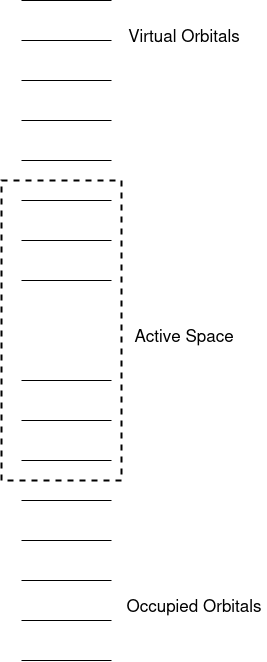
\includegraphics[scale=0.5]{Figures/CAS.png}
    \caption{Complete Active Space}
    \label{fig:enter-label}
\end{figure}

Within this active space, we can consider all possible excitations and since we're only choosing a small number of orbitals to work with, the number of excitations is not too large to perform our calculations. We can perform MCSCF calculations within this Active Space using all excitations, this is known as the Complete Active Space Self Consistent Field (CASSCF). Instead, if we perform a full CI calculation within the complete active space, it's called Complete Active Space Configuration Interaction or CASCI. We can also use the CASSCF result as a reference for performing 2nd or 4th order  M{\o}ller-Plesset perturbation theory calculations, which are the CASPT2 methods. 

One method that leverages the active space idea but reduces computational cost is the family of Reduced Active Space RASSCF methods. Instead of treating the entire space completely, we can divide the space into three parts, where we treat one part completely and consider only some excitations into and out of this part.

% RASSCF diagram.


When attempting to study exciting processes in organic photovoltaic materials such as multi-exciton generation, methods such as CIS and TD-DFT fail to capture these effects and that's where we find the CASSCF and related methods particularly helpful \cite{zimmerman2013correlated}.




\section{Phonons}

% What are phonons

% Sample phonon dispersion in a solid.

% How to get phonons from electronic structure calculations in solids (phonopy or something of that order).

% Why treating el-ph interactions in solids is important.



